% Dissertação de mestrado profissional em Biblioteconomia
% Modelo do ÉguaTex (https://www.eguatex.com.br), em domínio público pela licença CC0 1.0:
% use, modifique e distribua sem pedir permissão e sem citar a origem.
%
% Compile com pdfLaTeX e BibTeX (o ÉguaTex faz isso sozinho).
% Arquivos: main.tex (preâmbulo e elementos pré-textuais), capitulos/*.tex (um arquivo por
% capítulo, apêndice ou anexo) e referencias.bib (bibliografia).
% A ordem dos elementos segue a ABNT NBR 14724:2011.

\documentclass[
  12pt,         % corpo 12 pt, como pede a NBR 14724
  oneside,      % impressão só no anverso; troque por twoside para frente e verso
  a4paper,
  english,      % idioma do abstract
  brazil        % o último idioma é o principal (o abntex2 usa o nome brazil)
]{abntex2}

% ---------- fontes e codificação ----------
\usepackage[T1]{fontenc}
\usepackage[utf8]{inputenc}
\usepackage{tgtermes}           % texto com desenho de Times
\usepackage{tgheros}            % títulos sem serifa com desenho de Helvetica
\usepackage{microtype}
\usepackage{indentfirst}

% ---------- tabelas, figuras e cores ----------
\usepackage{booktabs}
\usepackage{tabularx}
\usepackage{xcolor}
\usepackage{tikz}
\usetikzlibrary{positioning, arrows.meta, shapes.geometric, babel}
\usepackage{enumitem}
\definecolor{azulbib}{RGB}{24,70,120}

% ---------- links e citações ABNT (hyperref antes do abntex2cite) ----------
\usepackage[alf]{abntex2cite}

% ---------- quadros (texto em células), com lista própria ----------
\newcommand{\quadroname}{Quadro}
\newcommand{\listofquadrosname}{Lista de quadros}
\newfloat[chapter]{quadro}{loq}{\quadroname}
\newlistof{listofquadros}{loq}{\listofquadrosname}
\newlistentry{quadro}{loq}{0}
\setfloatadjustment{quadro}{\centering}
\counterwithout{quadro}{chapter}
\renewcommand{\cftquadroname}{\quadroname\space}
\renewcommand*{\cftquadroaftersnum}{\hfill--\hfill}

% ---------- instruções de preenchimento ----------
% Os textos em cinza explicam o que escrever em cada parte.
% Troque \instrucoestrue por \instrucoesfalse para esconder todos de uma vez.
\newif\ifinstrucoes
\instrucoestrue
\newcommand{\instrucao}[1]{\ifinstrucoes{\color{gray}\small\itshape #1\par}\fi}

% ---------- dados do trabalho: preencha aqui ----------
\titulo{Guia de política de desenvolvimento de coleções para bibliotecas escolares da rede pública}
\autor{Nome do autor}
\local{Cidade}
\data{Ano}
\orientador{Prof.ª Dr.ª Nome da orientadora}
\coorientador{Prof. Dr. Nome do coorientador}
\instituicao{%
  Universidade Federal Exemplo
  \par
  Instituto de Ciências Sociais Aplicadas
  \par
  Programa de Pós-Graduação em Biblioteconomia (Mestrado Profissional)}
\tipotrabalho{Dissertação (Mestrado Profissional)}
\preambulo{Dissertação apresentada ao Programa de Pós-Graduação em Biblioteconomia da Universidade Federal Exemplo, como requisito parcial para a obtenção do título de Mestre em Biblioteconomia. Área de concentração: Gestão de unidades de informação.}

\makeatletter
\hypersetup{
  pdftitle={\@title},
  pdfauthor={\@author},
  pdfsubject={\imprimirpreambulo},
  colorlinks=true, linkcolor=azulbib, citecolor=azulbib, urlcolor=azulbib,
  bookmarksdepth=4
}
\makeatother

% Recuo de parágrafo e espaço entre parágrafos.
\setlength{\parindent}{1.25cm}
\setlength{\parskip}{0.2cm}

\begin{document}
\selectlanguage{brazil}
\frenchspacing

% ======================================================================
% Elementos pré-textuais (NBR 14724:2011, seção 4.2.1)
% ======================================================================

% Capa (obrigatória)
\imprimircapa

% Folha de rosto (obrigatória); o asterisco imprime a ficha catalográfica no verso
\imprimirfolhaderosto*

% Ficha catalográfica (verso da folha de rosto)
% Peça a ficha definitiva à biblioteca da universidade; o quadro abaixo é só a forma.
\begin{fichacatalografica}
  \sffamily
  \vspace*{\fill}
  \begin{center}
    {\small Dados Internacionais de Catalogação na Publicação (CIP)}\par\medskip
    \fbox{\begin{minipage}[c][7.5cm]{13.5cm}
      \small
      Sobrenome, Nome do autor.\par
      \hspace{0.5cm}\imprimirtitulo\ / Nome do autor. -- \imprimirlocal, \imprimirdata.\par
      \hspace{0.5cm}\thelastpage\ f. : il.\par\medskip
      \hspace{0.5cm}Orientadora: \imprimirorientador.\par
      \hspace{0.5cm}\imprimirtipotrabalho\ -- Universidade Federal Exemplo, Programa de Pós-Graduação em Biblioteconomia, \imprimirdata.\par\medskip
      \hspace{0.5cm}1. Desenvolvimento de coleções. 2. Biblioteca escolar. 3. Política de informação. I. Título.\par
      \vfill\hfill CDD 025.21
    \end{minipage}}
  \end{center}
\end{fichacatalografica}

% Errata (opcional): use só se a versão impressa já tiver sido entregue com erros.
\begin{errata}
  \instrucao{Elemento opcional, inserido depois da folha de rosto. Traga a referência do trabalho e uma tabela com folha, linha, onde se lê e leia-se. Apague o ambiente se não houver erros.}
  Sobrenome, Nome do autor. \textbf{\imprimirtitulo}. Ano. Dissertação (Mestrado Profissional em Biblioteconomia) -- Universidade Federal Exemplo, Cidade, Ano.

  \begin{table}[htb]
    \centering\small
    \begin{tabular}{cccc}
      \toprule
      \textbf{Folha} & \textbf{Linha} & \textbf{Onde se lê} & \textbf{Leia-se} \\
      \midrule
      32 & 12 & catalogacão & catalogação \\
      \bottomrule
    \end{tabular}
  \end{table}
\end{errata}

% Folha de aprovação (obrigatória)
\begin{folhadeaprovacao}
  \begin{center}
    {\ABNTEXchapterfont\large\imprimirautor}

    \vspace*{\fill}
    {\ABNTEXchapterfont\bfseries\Large\imprimirtitulo}
    \vspace*{\fill}

    \hspace{.45\textwidth}
    \begin{minipage}{.5\textwidth}
      \small\imprimirpreambulo
    \end{minipage}%
    \vspace*{\fill}
  \end{center}

  Aprovada em: dia de mês de Ano.

  \assinatura{\textbf{\imprimirorientador} (orientadora)\\ Universidade Federal Exemplo}
  \assinatura{\textbf{Prof. Dr. Nome do membro interno}\\ Universidade Federal Exemplo}
  \assinatura{\textbf{Prof.ª Dr.ª Nome da membra externa}\\ Instituição de origem}
\end{folhadeaprovacao}

% Dedicatória (opcional)
\begin{dedicatoria}
  \vspace*{\fill}
  \begin{flushright}
    \begin{minipage}{.5\textwidth}
      \itshape Aos bibliotecários e às bibliotecárias que mantêm abertas as bibliotecas das escolas públicas.
    \end{minipage}
  \end{flushright}
\end{dedicatoria}

% Agradecimentos (opcional)
\begin{agradecimentos}
  \instrucao{Elemento opcional. Agradeça em poucos parágrafos a quem contribuiu de forma direta: orientação, agência de fomento (com o número do processo), escolas participantes e colegas.}
  À orientadora, pela leitura atenta de cada versão.

  Às equipes das escolas que abriram as bibliotecas para a pesquisa e testaram o guia.

  Este trabalho teve apoio da agência de fomento pelo processo nº 000000/Ano.
\end{agradecimentos}

% Epígrafe (opcional)
\begin{epigrafe}
  \vspace*{\fill}
  \begin{flushright}
    \textit{``Every reader his book.''}\\
    % Em citação direta, acrescente a página: \cite[p.~xx]{chave}.
    \cite{ranganathan1931}
  \end{flushright}
\end{epigrafe}

% Resumo na língua do texto (obrigatório)
\setlength{\absparsep}{18pt}
\begin{resumo}
  \instrucao{Parágrafo único de 150 a 500 palavras (NBR 6028:2021): objetivo, método, resultados e conclusões. No mestrado profissional, diga também qual é o produto técnico e onde ele foi aplicado.}
  Esta dissertação apresenta um guia de política de desenvolvimento de coleções para bibliotecas escolares da rede pública municipal. A pesquisa, de abordagem qualitativa e natureza aplicada, combinou análise documental, questionário com profissionais de doze bibliotecas e oficinas de validação. O diagnóstico mostrou acervos sem critérios escritos de seleção e de descarte. O produto técnico, apresentado no Apêndice~\ref{ap:produto}, organiza esses critérios em etapas e formulários de uso imediato. A validação indicou que o guia é aplicável por equipes pequenas e sem formação específica.

  \textbf{Palavras-chave}: desenvolvimento de coleções. biblioteca escolar. política de informação. produto técnico.
\end{resumo}

% Resumo em língua estrangeira (obrigatório)
\begin{resumo}[Abstract]
  \begin{otherlanguage*}{english}
    This dissertation presents a collection development policy guide for public school libraries. The applied, qualitative study combined document analysis, a survey of staff at twelve libraries and validation workshops. The guide, presented in Appendix~\ref{ap:produto}, sets out selection and weeding criteria in steps and ready to use forms.

    \textbf{Keywords}: collection development. school library. information policy. technical product.
  \end{otherlanguage*}
\end{resumo}

% Listas (opcionais): ilustrações, quadros, tabelas, siglas e símbolos
\pdfbookmark[0]{\listfigurename}{lof}
\listoffigures*
\cleardoublepage
\pdfbookmark[0]{\listofquadrosname}{loq}
\listofquadros*
\cleardoublepage
\pdfbookmark[0]{\listtablename}{lot}
\listoftables*
\cleardoublepage

\begin{siglas}
  \item[ABNT] Associação Brasileira de Normas Técnicas
  \item[CDD] Classificação Decimal de Dewey
  \item[PDC] Política de Desenvolvimento de Coleções
  \item[PNLD] Programa Nacional do Livro e do Material Didático
\end{siglas}

% Lista de símbolos: elemento opcional; apague o ambiente se o trabalho não usar símbolos.
\begin{simbolos}
  \item[$n$] Número de bibliotecas participantes
  \item[$f_i$] Frequência absoluta da categoria $i$
  \item[$\%$] Percentual sobre o total de respostas
\end{simbolos}

% Sumário (obrigatório)
\pdfbookmark[0]{\contentsname}{toc}
\tableofcontents*
\cleardoublepage

% ======================================================================
% Elementos textuais
% ======================================================================
\textual
% ----------------------------------------------------------------------
% Capítulo 1: Introdução
% ----------------------------------------------------------------------
\chapter{Introdução}
\label{cap:introducao}

\instrucao{De três a cinco páginas. Apresente o problema prático que motivou o trabalho, o contexto profissional em que ele aparece, os objetivos e a estrutura da dissertação. No mestrado profissional, deixe claro desde o início qual produto técnico será entregue.}

As bibliotecas escolares da rede pública recebem livros de várias fontes ao mesmo tempo: programas federais, doações da comunidade e compras pontuais da escola. Sem uma política escrita, a seleção depende de quem está no balcão naquele ano, e o descarte quase nunca acontece. A Lei nº 12.244, de 24 de maio de 2010, ao tratar da universalização das bibliotecas escolares, reforçou a necessidade de acervos organizados e atualizados \cite{brasil2010}.

\section{Problema}
\instrucao{Escreva o problema em uma frase interrogativa, ligada à prática. Exemplo: como sistematizar critérios de seleção e descarte que equipes pequenas consigam aplicar?}

Como sistematizar critérios de seleção, aquisição, avaliação e descarte que as equipes das bibliotecas escolares municipais consigam aplicar sem apoio externo permanente?

\section{Objetivos}
\subsection{Objetivo geral}
Elaborar e validar um guia de política de desenvolvimento de coleções para bibliotecas escolares da rede pública municipal.

\subsection{Objetivos específicos}
\instrucao{Use verbos no infinitivo que possam ser verificados ao final: diagnosticar, elaborar, validar, propor.}
\begin{enumerate}[label=\alph*)]
  \item diagnosticar as práticas de formação de acervo das bibliotecas participantes;
  \item identificar, na literatura, os elementos mínimos de uma política de desenvolvimento de coleções;
  \item elaborar o guia como produto técnico;
  \item validar o guia com as equipes, em oficinas.
\end{enumerate}

\section{Justificativa}
\instrucao{Mostre a relevância para a instituição e para a área. No mestrado profissional, o impacto esperado do produto conta tanto quanto a lacuna teórica.}

A política escrita reduz decisões improvisadas, dá transparência ao uso de recursos públicos e protege a biblioteca diante de doações inadequadas. O guia proposto pode ser adotado por outras redes com ajustes mínimos.

\section{Estrutura do trabalho}
O Capítulo~\ref{cap:referencial} reúne os fundamentos. O Capítulo~\ref{cap:metodologia} descreve o percurso metodológico. O Capítulo~\ref{cap:diagnostico} apresenta o diagnóstico e a validação do produto. O Capítulo~\ref{cap:consideracoes} traz as considerações finais. O guia completo está no Apêndice~\ref{ap:produto}. A apresentação segue a NBR 14724 \cite{NBR14724:2011}, e as referências seguem a NBR 6023 \cite{NBR6023:2018}.

% ----------------------------------------------------------------------
% Capítulo 2: Referencial teórico
% ----------------------------------------------------------------------
\chapter{Referencial teórico}
\label{cap:referencial}

\instrucao{De oito a quinze páginas. Organize por conceitos, não por autores. Cada seção termina dizendo o que aquele conceito traz para o produto. Cite com \textbackslash cite e \textbackslash citeonline, no sistema autor-data da NBR 10520:2023.}

\section{Desenvolvimento de coleções como processo}
\instrucao{Defina o conceito e descreva as etapas do processo. Uma figura ajuda o leitor a ver o ciclo inteiro.}

O desenvolvimento de coleções é um processo contínuo, em que cada etapa alimenta a seguinte. A Figura~\ref{fig:ciclo} resume as seis etapas mais citadas na literatura da área, da análise da comunidade ao desbaste.

\begin{figure}[htb]
  \centering
  \caption{Etapas do desenvolvimento de coleções}
  \label{fig:ciclo}
  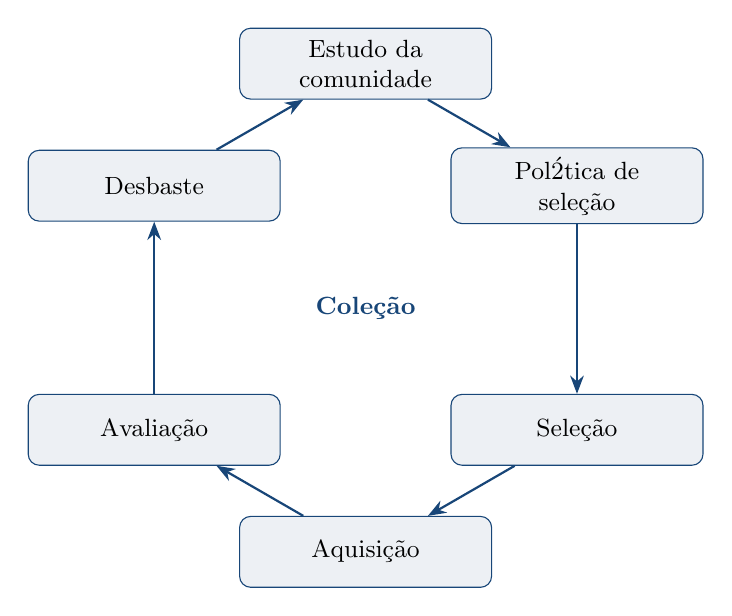
\begin{tikzpicture}[
      etapa/.style={draw=azulbib, fill=azulbib!8, rounded corners, minimum width=3.2cm,
        minimum height=0.9cm, align=center, font=\small},
      seta/.style={-{Stealth}, thick, azulbib}]
    \foreach \nome [count=\i] in {Estudo da\\comunidade, Política de\\seleção, Seleção, Aquisição, Avaliação, Desbaste}{
      \node[etapa] (e\i) at ({90-(\i-1)*60}:3.1cm) {\nome};
    }
    \foreach \i/\j in {1/2,2/3,3/4,4/5,5/6,6/1}{
      \draw[seta] (e\i) -- (e\j);
    }
    \node[font=\small\bfseries, text=azulbib] {Coleção};
  \end{tikzpicture}
  \fonte{Elaborada pelo autor.}
\end{figure}

\section{As leis da Biblioteconomia}
\instrucao{Relacione um princípio clássico com o problema. Exemplo: a segunda lei justifica que a seleção parta do perfil dos leitores.}

As cinco leis formuladas por \citeonline{ranganathan1931} continuam úteis como critério de avaliação de acervos. A segunda lei, \textit{every reader his book}, orienta a seleção a partir do perfil dos leitores. A quinta, \textit{a library is a growing organism}, sustenta a necessidade de prever o crescimento e o desbaste no mesmo documento.

\section{Política de desenvolvimento de coleções}
\instrucao{Liste os elementos mínimos de uma política, de preferência num quadro. Esses elementos viram as seções do produto.}

O Quadro~\ref{qua:elementos} reúne os elementos que o guia deve conter.

\begin{quadro}[htb]
  \caption{Elementos mínimos de uma política de desenvolvimento de coleções}
  \label{qua:elementos}
  \small
  \begin{tabularx}{\textwidth}{lX}
    \toprule
    \textbf{Elemento} & \textbf{O que define} \\
    \midrule
    Objetivos & A missão da biblioteca e o público atendido \\
    Seleção & Critérios de qualidade, pertinência e atualidade \\
    Aquisição & Compra, permuta e doação, com regras para cada via \\
    Avaliação & Indicadores de uso e periodicidade da revisão \\
    Desbaste & Critérios de remanejamento e descarte \\
    \bottomrule
  \end{tabularx}
  \fonte{Elaborado pelo autor.}
\end{quadro}

\section{Produto técnico no mestrado profissional}
\instrucao{Explique o que caracteriza um produto técnico (aplicabilidade, replicabilidade, impacto) e como ele será avaliado. Consulte o regulamento do seu programa.}

No mestrado profissional, a dissertação descreve a pesquisa que fundamenta um produto de uso imediato no ambiente de trabalho. Neste estudo, o produto é um guia com textos-modelo e formulários, que a escola adapta e aprova como política própria.

% ----------------------------------------------------------------------
% Capítulo 3: Procedimentos metodológicos
% ----------------------------------------------------------------------
\chapter{Procedimentos metodológicos}
\label{cap:metodologia}

\instrucao{De quatro a oito páginas. Classifique a pesquisa (abordagem, natureza, objetivos, procedimentos), descreva o campo, os participantes, os instrumentos e as etapas de elaboração e validação do produto. Escreva no passado.}

\section{Caracterização da pesquisa}
A pesquisa é aplicada quanto à natureza, qualitativa quanto à abordagem e descritiva quanto aos objetivos. Os procedimentos combinaram análise documental, levantamento por questionário e oficinas de validação.

\section{Campo e participantes}
\instrucao{Informe quantos locais e quantas pessoas participaram, como foram escolhidos e o parecer do comitê de ética, quando houver.}

Participaram as equipes de doze bibliotecas escolares, escolhidas por conveniência entre as unidades com profissional fixo. A pesquisa seguiu a Resolução CNS nº 510/2016 \cite{brasil2016}.

\section{Etapas}
\instrucao{Descreva as etapas na ordem em que aconteceram, com o produto de cada uma.}
\begin{enumerate}[label=\arabic*)]
  \item análise de documentos das escolas (regimentos, inventários e termos de doação);
  \item aplicação do questionário do Apêndice~\ref{ap:questionario};
  \item redação da primeira versão do guia;
  \item duas oficinas de validação, com registro das sugestões;
  \item redação da versão final, avaliada com a ficha do Anexo~\ref{an:ficha}.
\end{enumerate}

\section{Análise dos dados}
As respostas abertas foram agrupadas em categorias definidas a partir dos elementos do Quadro~\ref{qua:elementos}. As respostas fechadas foram resumidas em frequências absolutas e percentuais.

% ----------------------------------------------------------------------
% Capítulo 4: Diagnóstico e validação do produto
% ----------------------------------------------------------------------
\chapter{Diagnóstico e validação do produto}
\label{cap:diagnostico}

\instrucao{De oito a quinze páginas. Primeiro os resultados do diagnóstico, depois a descrição do produto e, por fim, a validação. Cada tabela ou figura é citada no texto antes de aparecer.}

\section{Diagnóstico das bibliotecas}
A Tabela~\ref{tab:praticas} resume as práticas declaradas pelas equipes (dados de exemplo).

\begin{table}[htb]
  \centering
  \caption{Práticas de formação de acervo declaradas ($n = 12$)}
  \label{tab:praticas}
  \begin{tabular}{lrr}
    \toprule
    \textbf{Prática} & \textbf{$f_i$} & \textbf{\%} \\
    \midrule
    Possui critérios escritos de seleção & 2 & 16,7 \\
    Registra as doações recebidas & 7 & 58,3 \\
    Fez descarte nos últimos três anos & 3 & 25,0 \\
    Consulta os leitores antes de comprar & 5 & 41,7 \\
    \bottomrule
  \end{tabular}
  \fonte{Dados da pesquisa (exemplo).}
\end{table}

\instrucao{Interprete a tabela em vez de repeti-la. Exemplo: o dado mais baixo aponta a seção do guia que precisa de mais detalhe.}
O dado que mais chama atenção é a ausência de critérios escritos em dez das doze bibliotecas. Esse resultado definiu a seção de seleção como a parte mais detalhada do guia.

\section{Descrição do produto}
\instrucao{Apresente o produto: público, formato, seções e modo de uso. O produto completo vai no apêndice; aqui entra a visão geral.}

O guia tem cinco seções, uma para cada elemento do Quadro~\ref{qua:elementos}, e quatro formulários. Cada seção traz um texto-modelo que a escola completa com seus dados e aprova no conselho escolar.

\section{Validação}
\instrucao{Relate como o produto foi testado, quem avaliou, quais critérios foram usados e o que mudou na versão final.}

As oficinas reuniram as equipes das doze bibliotecas. As sugestões mais frequentes foram simplificar o formulário de doação e incluir exemplos de justificativa de descarte, ambas incorporadas à versão final.

% ----------------------------------------------------------------------
% Capítulo 5: Considerações finais
% ----------------------------------------------------------------------
\chapter{Considerações finais}
\label{cap:consideracoes}

\instrucao{De duas a quatro páginas. Retome cada objetivo específico e diga como foi atingido. Aponte limitações, o impacto esperado do produto e sugestões de continuidade. Não traga dados novos.}

O diagnóstico confirmou que a falta de critérios escritos é o principal obstáculo à gestão dos acervos escolares da rede. O guia elaborado responde a esse problema com textos-modelo e formulários simples, e a validação indicou que as equipes conseguem aplicá-lo sem apoio externo.

A pesquisa se limitou a bibliotecas com profissional fixo. Estudos futuros podem testar o guia em unidades atendidas por professores readaptados e acompanhar, ao longo de dois anos, os efeitos da política sobre o uso do acervo.


% ======================================================================
% Elementos pós-textuais
% ======================================================================
\postextual
\bibliography{referencias}

\begin{apendicesenv}
  \partapendices
  % ----------------------------------------------------------------------
% Apêndice A: o produto técnico
% Apêndice é material elaborado pelo próprio autor (NBR 14724:2011, 4.2.3.3).
% ----------------------------------------------------------------------
\chapter{Produto técnico: guia de política de desenvolvimento de coleções}
\label{ap:produto}

\instrucao{Coloque aqui o produto completo, no formato em que será entregue à instituição. Se ele tiver identidade visual própria, mantenha a página de rosto do produto e a ficha técnica. Produtos em outro suporte (vídeo, sistema, site) entram com descrição, endereço de acesso e capturas de tela.}

\begin{center}
  \fcolorbox{azulbib}{azulbib!6}{\begin{minipage}{0.86\textwidth}
    \centering\vspace{1em}
    {\large\bfseries\color{azulbib} Guia de política de desenvolvimento de coleções\par}
    \medskip
    {Bibliotecas escolares da rede pública municipal\par}
    \medskip
    {\small Nome do autor e Nome da orientadora\par Cidade, Ano\par}
    \vspace{1em}
  \end{minipage}}
\end{center}

\section*{Ficha técnica}
\noindent\begin{tabularx}{\textwidth}{@{}lX@{}}
  Tipo de produto & Manual técnico com formulários \\
  Público & Equipes de bibliotecas escolares \\
  Registro & ISBN ou repositório institucional, quando houver \\
  Licença & Indique a licença de uso, por exemplo CC BY 4.0 \\
\end{tabularx}

\section*{1 Objetivos da política}
\instrucao{Texto-modelo que a escola completa: missão da biblioteca, público e níveis de ensino atendidos.}
A biblioteca da Escola \underline{\hspace{4cm}} atende estudantes do ensino fundamental, professores e comunidade, e tem por missão apoiar o currículo e incentivar a leitura.

\section*{2 Critérios de seleção}
\begin{enumerate}[label=\alph*)]
  \item adequação à faixa etária e ao currículo;
  \item qualidade do conteúdo e da edição;
  \item atualidade, nas áreas em que a informação envelhece depressa;
  \item demanda registrada no livro de sugestões.
\end{enumerate}

\section*{3 Doações}
Toda doação é recebida mediante termo, e a biblioteca decide se incorpora, repassa ou descarta o material segundo os critérios da seção 2.

\section*{4 Avaliação e desbaste}
O acervo é avaliado a cada dois anos. Materiais desatualizados, danificados ou sem empréstimo há cinco anos são remanejados ou descartados, com registro em formulário próprio.

\section*{Formulário 1: termo de doação}
\noindent Doador(a): \hrulefill\par\smallskip
\noindent Quantidade de itens: \underline{\hspace{2cm}}\quad Data: \underline{\hspace{3cm}}\par\smallskip
\noindent Declaro estar ciente de que a biblioteca decidirá sobre a destinação dos itens.\par\bigskip
\noindent\hfill\rule{6cm}{0.4pt}\par
\noindent\hfill Assinatura do doador

  % ----------------------------------------------------------------------
% Apêndice B: instrumento de coleta
% ----------------------------------------------------------------------
\chapter{Questionário aplicado às equipes}
\label{ap:questionario}

\instrucao{Reproduza o instrumento exatamente como foi aplicado, com o texto de apresentação e as instruções ao respondente.}

\textbf{Apresentação.} Este questionário faz parte de uma pesquisa de mestrado sobre a formação de acervos em bibliotecas escolares. As respostas são anônimas.

\begin{enumerate}[label=\arabic*.]
  \item A biblioteca possui critérios escritos para a seleção de materiais?\\
    ( ) Sim \quad ( ) Não \quad ( ) Não sei
  \item As doações recebidas são registradas?\\
    ( ) Sempre \quad ( ) Às vezes \quad ( ) Nunca
  \item Quando foi feito o último descarte de materiais?\\
    ( ) Há menos de um ano \quad ( ) Entre um e três anos \quad ( ) Há mais de três anos \quad ( ) Nunca
  \item Descreva como a biblioteca decide o que comprar.\\[0.5em]
    \rule{\linewidth}{0.4pt}\\[0.8em]\rule{\linewidth}{0.4pt}
\end{enumerate}

\end{apendicesenv}

\begin{anexosenv}
  \partanexos
  % ----------------------------------------------------------------------
% Anexo A: documento de terceiros
% Anexo é material não elaborado pelo autor (NBR 14724:2011, 4.2.3.4).
% ----------------------------------------------------------------------
\chapter{Ficha de avaliação do produto técnico}
\label{an:ficha}

\instrucao{Anexe documentos de outros autores que fundamentam o trabalho: a ficha de avaliação de produtos do programa, normas internas, termos de anuência das escolas. Indique a fonte de cada documento. Reproduza o original ou transcreva-o, como no exemplo.}

\begin{table}[htb]
  \centering
  \small
  \begin{tabularx}{\textwidth}{Xcccc}
    \toprule
    \textbf{Critério} & \textbf{1} & \textbf{2} & \textbf{3} & \textbf{4} \\
    \midrule
    Aderência à linha de pesquisa & ( ) & ( ) & ( ) & ( ) \\
    Aplicabilidade no ambiente de trabalho & ( ) & ( ) & ( ) & ( ) \\
    Replicabilidade em outras instituições & ( ) & ( ) & ( ) & ( ) \\
    Inovação & ( ) & ( ) & ( ) & ( ) \\
    Complexidade de elaboração & ( ) & ( ) & ( ) & ( ) \\
    \bottomrule
  \end{tabularx}
  \fonte{Programa de Pós-Graduação em Biblioteconomia (exemplo).}
\end{table}

\noindent Escala: 1 = insuficiente; 2 = regular; 3 = bom; 4 = excelente.

\end{anexosenv}

\end{document}
